%%%%%%%%%%%%%%%%%%%%%%%%%%%%%%%%%%%%%%%%%12pt: grandezza carattere
                                        %a4paper: formato a4
                                        %openright: apre i capitoli a destra
                                        %twoside: serve per fare un
                                        %   documento fronteretro
                                        %report: stile tesi (oppure book)
\documentclass[12pt,a4paper,openright,twoside]{report}
%
%%%%%%%%%%%%%%%%%%%%%%%%%%%%%%%%%%%%%%%%%libreria per scrivere in italiano
\usepackage[italian]{babel}
\usepackage{listings}
%
%%%%%%%%%%%%%%%%%%%%%%%%%%%%%%%%%%%%%%%%%libreria per accettare i caratteri
                                        %   digitati da tastiera come � �
                                        %   si pu� usare anche
                                        %   \usepackage[T1]{fontenc}
                                        %   per� con questa libreria
                                        %   il tempo di compilazione
                                        %   aumenta
\usepackage[latin1]{inputenc}
%
%%%%%%%%%%%%%%%%%%%%%%%%%%%%%%%%%%%%%%%%%libreria per impostare il documento
\usepackage{fancyhdr}
%
%%%%%%%%%%%%%%%%%%%%%%%%%%%%%%%%%%%%%%%%%libreria per avere l'indentazione
%%%%%%%%%%%%%%%%%%%%%%%%%%%%%%%%%%%%%%%%%   all'inizio dei capitoli, ...
\usepackage{indentfirst}
%
%%%%%%%%%libreria per mostrare le etichette
%\usepackage{showkeys}
%
%%%%%%%%%%%%%%%%%%%%%%%%%%%%%%%%%%%%%%%%%libreria per inserire grafici
\usepackage{graphicx}
\graphixpath{ ./images/ }
%
%%%%%%%%%%%%%%%%%%%%%%%%%%%%%%%%%%%%%%%%%libreria per utilizzare font
                                        %   particolari ad esempio
                                        %   \textsc{}
\usepackage{newlfont}
%
%%%%%%%%%%%%%%%%%%%%%%%%%%%%%%%%%%%%%%%%%librerie matematiche
\usepackage{amssymb}
\usepackage{amsmath}
\usepackage{latexsym}
\usepackage{amsthm}
%
\oddsidemargin=30pt \evensidemargin=20pt%impostano i margini
\hyphenation{sil-la-ba-zio-ne pa-ren-te-si}%serve per la sillabazione: tra parentesi
					   %vanno inserite come nell'esempio le parole
%					   %che latex non riesce a tagliare nel modo giusto andando a capo.

%
%%%%%%%%%%%%%%%%%%%%%%%%%%%%%%%%%%%%%%%%%comandi per l'impostazione
                                        %   della pagina, vedi il manuale
                                        %   della libreria fancyhdr
                                        %   per ulteriori delucidazioni
\pagestyle{fancy}\addtolength{\headwidth}{20pt}
\renewcommand{\chaptermark}[1]{\markboth{\thechapter.\ #1}{}}
\renewcommand{\sectionmark}[1]{\markright{\thesection \ #1}{}}
\rhead[\fancyplain{}{\bfseries\leftmark}]{\fancyplain{}{\bfseries\thepage}}
\cfoot{}
%%%%%%%%%%%%%%%%%%%%%%%%%%%%%%%%%%%%%%%%%
\linespread{1.3}                        %comando per impostare l'interlinea
%%%%%%%%%%%%%%%%%%%%%%%%%%%%%%%%%%%%%%%%%definisce nuovi comandi
%
\begin{document}
\begin{titlepage}                       %crea un ambiente libero da vincoli
                                        %   di margini e grandezza caratteri:
                                        %   si pu\`o modificare quello che si
                                        %   vuole, tanto fuori da questo
                                        %   ambiente tutto viene ristabilito
%
\thispagestyle{empty}                   %elimina il numero della pagina
\topmargin=6.5cm                        %imposta il margina superiore a 6.5cm
\raggedleft                             %incolonna la scrittura a destra
\large                                  %aumenta la grandezza del carattere
                                        %   a 14pt
\em                                     %emfatizza (corsivo) il carattere
Alla mia famiglia, \\
che mi ha sempre sostenuto \\
in ogni mia scelta.                      %\ldots lascia tre puntini
\newpage                                %va in una pagina nuova
%
%%%%%%%%%%%%%%%%%%%%%%%%%%%%%%%%%%%%%%%%
\clearpage{\pagestyle{empty}\cleardoublepage}%non numera l'ultima pagina sinistra
\end{titlepage}
\pagenumbering{roman}                   %serve per mettere i numeri romani
\chapter*{Introduzione}                 %crea l'introduzione (un capitolo
                                        %   non numerato)
%%%%%%%%%%%%%%%%%%%%%%%%%%%%%%%%%%%%%%%%%imposta l'intestazione di pagina
\rhead[\fancyplain{}{\bfseries
INTRODUZIONE}]{\fancyplain{}{\bfseries\thepage}}
\lhead[\fancyplain{}{\bfseries\thepage}]{\fancyplain{}{\bfseries
INTRODUZIONE}}
%%%%%%%%%%%%%%%%%%%%%%%%%%%%%%%%%%%%%%%%%aggiunge la voce Introduzione
                                        %   nell'indice
\addcontentsline{toc}{chapter}{Introduzione}
Questa \`e l'introduzione.
%%%%%%%%%%%%%%%%%%%%%%%%%%%%%%%%%%%%%%%%%non numera l'ultima pagina sinistra
\clearpage{\pagestyle{empty}\cleardoublepage}
\tableofcontents                        %crea l'indice
%%%%%%%%%%%%%%%%%%%%%%%%%%%%%%%%%%%%%%%%%imposta l'intestazione di pagina
\rhead[\fancyplain{}{\bfseries\leftmark}]{\fancyplain{}{\bfseries\thepage}}
\lhead[\fancyplain{}{\bfseries\thepage}]{\fancyplain{}{\bfseries
INDICE}}
%%%%%%%%%%%%%%%%%%%%%%%%%%%%%%%%%%%%%%%%%non numera l'ultima pagina sinistra
\clearpage{\pagestyle{empty}\cleardoublepage}
\listoffigures                          %crea l'elenco delle figure
%%%%%%%%%%%%%%%%%%%%%%%%%%%%%%%%%%%%%%%%%non numera l'ultima pagina sinistra
\clearpage{\pagestyle{empty}\cleardoublepage}
\listoftables                           %crea l'elenco delle tabelle
%%%%%%%%%%%%%%%%%%%%%%%%%%%%%%%%%%%%%%%%%non numera l'ultima pagina sinistra
\clearpage{\pagestyle{empty}\cleardoublepage}
\chapter{Lo stato dell'Arte}                %crea il capitolo
%%%%%%%%%%%%%%%%%%%%%%%%%%%%%%%%%%%%%%%%%imposta l'intestazione di pagina
\lhead[\fancyplain{}{\bfseries\thepage}]{\fancyplain{}{\bfseries\rightmark}}
\pagenumbering{arabic}                  %mette i numeri arabi
In questo capitolo si va ad illustrare lo stato dell'Arte delle tecnologie utilizzate.
Si illustreranno le principali qualit\`a degli Intrusion Detection Systems e le caratteristiche
principali che hanno portato durante i test alla scelta di un software rispetto che un altro.
Si passer\`a poi a presentare sFlow, illustrandone i benefici e le principali differenze
con NetFlow e di come esso viene attualmente utilizzato per affiancare un IDS in reti
molto estese e complesse.
Infine si dar\`a una breve presentazione dello stack ELK, (Elasticsearch-Logstash-Kibana)
e di come esso sia utilizzato nell'ambito della Network Security.
\section{Intrusion Detection System}
Un Intrusion Detection System (IDS) \cite{K4} \`e un dispositivo o un' applicazione software
che monitora una rete o un sistema per rilevare eventuali attivit\`a dannose o violazioni
delle policy. Qualsiasi attivit\`a o violazione rilevata viene in genere segnalata
ad un amministratore o raccolta a livello centrale utilizzando un
Security Information and Event Management (SIEM).
Un SIEM combina output provenienti da pi\`u sorgenti e utilizza tecniche di filtraggio
degli allarmi per distinguere le attivit\`a dannose dai falsi allarmi.

Esiste un' ampia gamma di IDS, che varia dal software antivirus fino ai sistemi gerarchici
che controllano il traffico di un' intera backbone. La classificazione pi\`u comune
\`e tra:
\begin{itemize}
  \item {\bf Network-based Intrusion Detection Firmware (NIDS)}: ad esempio un sistema
  che monitora il traffico di rete passante attraverso alcuni punti strategici di una
  rete. Esempi famosi sono: Suricata \cite{K6} , Snort \cite{K7} e BRO \cite{K8} .
  \item {\bf Host-based Intrusion Detection (HIDS)} : ad esempio un software che monitora
  alcuni file importanti del sistema operativo su cui \`e installato. Un esempio famoso
  di HIDS \`e OSSec \cite{K5}
\end{itemize}

Il panorama degli Intrusion Detection System (IDS) \`e al giorno d'oggi in continua evoluzione.
Tuttavia \`e possibile operare una seconda e importante classificazione in base a due criteri
principali che ne determinano il funzionamento:
\begin{itemize}
  \item Sistemi {\it signature-based}
  \item Sistemi basati su {\it anomaly detection}
\end{itemize}

Un IDS {\it signature-based } analizza i pacchetti passanti su una rete utilizzando il concetto di {\it signature}:
Una signature \`e un pattern che corrisponde ad un tipo di attacco noto. \cite{K7}
Esempi di signature possono essere:
\begin{itemize}
  \item un tentativo di connessione a telnet con username "root", che corrisponde
  ad una violazione delle policy di sicurezza
  \item un email con oggetto "Immagini gratis!" e un allegato con nome "freepics.exe",
  che sono caratteristici di un attacco nostro
  \item tentativi ripetuti nel tempo di connessione ssh ad intervalli sospetti,
  che identificano un possibile attacco bruteforce su ssh.
\end{itemize}

Il rilevamento signature-based \`e molto efficace nel rilevare minacce note,
ma in gran parte inefficace nel rilevare minacce precedentemente sconosciute,
minacce mascherate dall'uso di tecniche di evasione e molte varianti di minacce note.
 Per esempio, se un aggressore ha modificato il malware nell' esempio precedente per
 usare un nome file di "freepics2.exe", una firma che cercava "freepics.exe" non lo
 corrisponderebbe.
Il rilevamento basato sulla firma \`e il metodo di rilevamento pi\`u semplice in
quanto confronta il campione corrente, come un pacchetto o una voce di registro,
con un elenco di firme utilizzando operazioni di confronto tra stringhe. 



Questo ci mette al riparo
da una grandissima quantit\`a di attacchi conosciuti e si \`e rilevato nel corso degli anni
un sistema efficiente e ampiamente utilizzato.

I secondi invece utilizzano tecniche di intelligenza artificiale per determinare se
un comportamento sia lecito oppure no basandosi su quello che \`e stato definito
in fase di installazione come uno "stato normale".

Sebbene nell'ultimo periodo l'intelligenza artificiale stia facendo la sua comparsa in ogni
ambito dell'informatica gli IDS signature based rappresentano tuttora un'importante
fetta (se non la maggioranza) degli IDS in uso nei pi\`u importanti data center del mondo
ed \`e per questo che vale la pena studiarli.

In questo elaborato ci si focalizzer\`a sugli IDS signature based e se ne analizzeranno
le loro prestazioni combinate ad altre tecnologie che verranno introdotte in seguito.

Come anticipato sopra, tra i maggiori esponenti degli IDS attualmente utilizzati abbiamo:
\begin{itemize}
  \item Snort: Un IDS sviluppato a partire dagli anni '90, acquisito da Cisco nel 2013 e
  che \`e tuttora il pi\`u utilizzato in ambito enterprise.
  \item Suricata: Un IDS del nuovo millennio, sviluppato a partire dal 2009 da
  Open Information Security Foundation (OISF) e che vanta molteplici vantaggi sopra gli altri IDS.
\end{itemize}

In questo elaborato si \`e preferito utilizzare per motivi di performance e di implementazione,
Suricata. I dettagli di questa scelta saranno chiari pi\`u avanti quando saranno state
introdotte le principali caratteristiche di Suricata.

\subsection{Suricata, una breve introduzione}
Suricata \`e un IDS che fa uso di pattern matching per il riconoscimento dei threat
capace di effettuare un'analisi dei pacchetti molto approfondita. Il funzionamento del pattern matching pu\`o
essere riassunto dalla figura 1.1. \cite{K2}
\begin{figure}
  \begin{center}                          %centra nel mezzo della pagina
    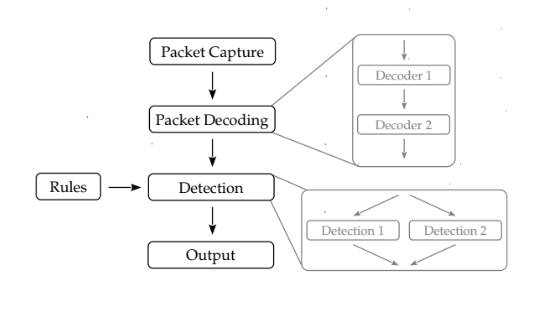
\includegraphics[width=90mm]{images/suricata-structure.png}
    \caption{Funzionamento del pattern matching}
    \label{}
  \end{center}
\end{figure}
Ogni pacchetto viene quindi decodificato e poi analizzato parallelamente per riscontrare
similitudini con pi\`u pattern.
E' stato dimostrato infatti (trovare il paper) che Suricata, data la sua natura multi threaded,
\`e di gran lunga pi\`u veloce di Snort (in ambienti multi-core), il quale invece \`e single thread.
Mentre una tipica regola per il suddetto patter matching \`e fatta in questo modo:
\begin{verbatim}
  rule header    alert tcp any any -> 192.168.1.0/24 111
\end{verbatim}
La praticit\`a dell'utilizzare questa sintassi sta nel fatto che essa \`e quasi del
tutto identica a quella di Snort. Per cui l'utilizzo dell'uno o dell'altro software,
almeno nel caso di studio di questa tesi, non \`e determinante.
E` possibile definire regole personalizzate, cos\`i come scaricarne di gi\`a confezionate
molto accurate.

Infine una delle caratteristiche fondamentali di Suricata sta nel fatto che esso pu\`o funzionare in
due modi distinti:
\begin{itemize}
  \item In modalit\`a online: viene monitorata una interfaccia specifica in modalita` promisqua,
  ossia tutti i pacchetti passanti per quella determinata interfaccia vengono decodificati e analizzati.
  \item In modalita offline: viene monitorato un file pcap contenente del traffico
  "registrato" in precedenza e che costituisce un punto di riferimento per l'analisi
  prestazionale delle regole o dell'istanza di Suricata da analizzare.
\end{itemize}

\section{sFlow}

sFlow \cite{K1} \`e una tecnologia per monitorare il traffico in reti contenenti
switches e routers che utilizza il capionamento di pacchetti. In particolare, esso
definisce i meccanismi di campionamento implementati
in un \emph{sFlow Agent} e il formato dei dati campionati mandati da tale Agent.

Il monitoraggio si compone di due elementi fondamentali:
\begin{itemize}
  \item {\bf sFlow Agent}: ovvero un qualsiasi apparato in grado di campionare
  i pacchetti secondo le specifiche di sFlow e di inviarli ad un {\it Collector}.
  l'Agent \`e un componente molto versatile ed estremamente performante dell'architettura
  sFlow che pu\`o essere impersonato anche da uno switch o da un router, senza degradarne
  le prestazioni.
  Il campionamento e la raccolta dei dati del nodo viene fatta in hardware e non presenta
  overhead nemmeno su reti Gigabit.
  \item {\bf Collector}: ovvero una macchina in qualsiasi parte del mondo in grado di raccogliere
  i dati sFlow e di elaborarli.
\end{itemize}

L'architettura e le modalit\`a di campionamento usati in sFlow offrono numerosi vantaggi
tra cui quello di avere una visione di tutta la rete ({\it network-wide}) in tempo
reale. Infatti, i pacchetti campionati vengono mandati al collector non appena arrivano
all'agent. Inoltre l'architettura \`e estremamente scalabile e permette di posizionare agent in diversi punti della rete,
o anche in reti diverse.

\newpage

\subsection{Campionamento}

Il campionamento \`e la parte fondamentale del protocollo sFlow, ed \`e anche
il motivo per cui esso si distacca da altre tecnologie simili come NetFlow.

Avvengono due tipi di campionamento:
\begin{itemize}
  \item un campionamento: in cui viene salvato 1 pacchetto ogni N, con N configurabile
  \item un troncamento: in cui il pacchetto designato per il salvataggio viene troncato,
  solitamente ad una dimensione di 128 Byte (tuttavia configurabile)
\end{itemize}

Questi due meccanismi insieme permettono di avere una visione della rete sufficientemente
accurata o comunque di una accuratezza configurabile.

\subsubsection{sFlow vs Netflow}

Un'altra tecnologia molto simile ad sFlow \`e NetFlow, sviluppato da Cisco.
Essi si differenziano per un motivo importantissimo e che non permette di usare efficacemente
NetFlow per monitorare la rete a fianco di un IDS; ovvero che Netflow fornisce solo
dati aggregati e non fornisce un troncamento parametrizzabile. Esso infatti esporta solo il Layer 3 del
pacchetto, questo fa perdere tutte le informazioni che, nel nostro particolare campo di applicazione,
sarebbero state utili, come l'header dei livelli superiori.

Qui \`e possibile vedere un esempio di un output del comando {\it nfdump}:
\begin{figure}[h!]
  \begin{center}                          %centra nel mezzo della pagina
    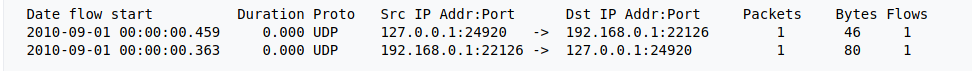
\includegraphics[width=\linewidth]{images/netflow.png}
    \caption{}
    \label{}
  \end{center}
\end{figure}

\newpage

\section{Packet sampling e IDS}

La sicurezza delle reti, specie di quelle molto estese, \`e un problema tutt'oggi
presente e di un importanza vitale in qualsiasi azienda che operi nel settore ICT (Information and Communications Technologies).
Le minacce possono avvenire in qualunque momento \cite{K3} ed essere generate sia dall'interno
che dall'esterno. Riuscire ad identificare queste minacce in tempo \`e il primo passo verso la soluzione di
questo difficile problema. Per fare ci\`o \`e necessario avere un'ampia e continua
sorveglianza della rete.
Storicamente la sorveglianza di una grande rete era (ed \`e tuttora) affidata a sonde ({\it probes}),
posizionate in punti strategici della rete. Questo \`e stato sufficientemente accurato
fino ad ora, quando si sta verificando un aumento dell'installazione di switched point to point network.
Quindi implementare il monitoraggio gi\`a dall'interno di uno switch o di router sta
diventando sempre pi\`u una necessit\`a. Tuttavia le esigenze di mercato tendono a preferire
l'ampiezza di banda sulla sicurezza, per cui la funzione di monitoraggio deve essere relegata come
funzione secondaria all'interno di questi apparati di rete. E` necessario quindi che questa funzione
operi con il minimo overhead possibile, al fine di non degradare le prestazioni dell'apparato.
E` qui che entra in gioco la tecnologia sFlow, essa permette di delegare la parte di analisi del traffico
ad un altro componente della rete ({\it il collector}), lasciando allo switch o al router le risorse per
effettuare le loro decisioni di smistamento dei pacchetti.

Vediamo allora come sflow garantisce l'efficacia del sistema di monitoraggio richiesto:
\begin{itemize}
  \item Sorveglianza continua network-wide: sFlow pu\`o essere configurato su ogni apparato di rete
  \item I dati devono essere sempre disponibili per rispondere efficacemente: sFlow manda immediatamente
  i pacchetti campionati al Collector con UDP
  \item I dati devono essere sufficientemente dettagliati per caratterizzare l'attacco: sFlow permette di
  esportare pi\`u di 128 Byte (comprendendo quindi ad esempio anche header di livello 7)
  \item Il sistema di monitoraggio non deve esporre gli apparato ad attacchi: sFlow impatta sulle
  prestazioni degli apparati poich\`e viene effettuato in hardware inoltre il consumo di banda \`e limitato
  poich\`e i datagram sFlow sono compressi
\end{itemize}

\newpage

\section{Stack ELK}

Lo stack ELK \`e uno stack formato dai tre programmi (Elasticsearch, Logstash e Kibana)
i quali uniti insieme forniscono una metodologia di centralizzazione, esplorazione
e visualizzazione dei log. Esso si compone di tre componenti fondamentali:
\begin{itemize}
  \item {\bf Logstash} : il quale si occupa di raccogliere i log, manipolarli cos\`i da renderli
  consumabili da elasticsearch
  \item {\bf Elasticsearch} : un database No-SQL particolarmente ottimizzato per la
  ricerca
  \item {\bf Kibana} : un visualizzatore dei dati contenuti in Elasticsearch che permette
  di effettuare ricerche e aggregare i dati in modo da fornirne una visualizzazione utile
  dei dati di log raccolti
\end{itemize}

Lo stack ELK \`e ad oggi lo standard {\it de facto} per l'esplorazione dei log,
esso si va ad affiancare a tutti i programmi critici all'interno di una infrastruttura
e risulta particolarmente utile nell'esplorazione dei log degli IDS. Esso permette infatti
acquisire in pochissimi secondi conoscenza su cosa accade nella rete e su che tipo di attacchi
sono in corso. I dati vengono fruiti all'operatore in maniera veloce e comprensibile tramite
dashboard, fornendo una fotografia estremamente informativa dello stato attuale

\newpage

%%%%%%%%%%%%%%%%%%%%%%%%%%%%%%%%%%%%%%%%%non numera l'ultima pagina sinistra
\clearpage{\pagestyle{empty}\cleardoublepage}
%%%%%%%%%%%%%%%%%%%%%%%%%%%%%%%%%%%%%%%%%per fare le conclusioni
\chapter*{Conclusioni}
%%%%%%%%%%%%%%%%%%%%%%%%%%%%%%%%%%%%%%%%%imposta l'intestazione di pagina
\rhead[\fancyplain{}{\bfseries
CONCLUSIONI}]{\fancyplain{}{\bfseries\thepage}}
\lhead[\fancyplain{}{\bfseries\thepage}]{\fancyplain{}{\bfseries
CONCLUSIONI}}
%%%%%%%%%%%%%%%%%%%%%%%%%%%%%%%%%%%%%%%%%aggiunge la voce Conclusioni
                                        %   nell'indice
\addcontentsline{toc}{chapter}{Conclusioni} Queste sono le
conclusioni.\\
In queste conclusioni voglio fare un riferimento alla
bibliografia: questo \`e il mio riferimento \cite{K3,K4}.
%%%%%%%%%%%%%%%%%%%%%%%%%%%%%%%%%%%%%%%%%imposta l'intestazione di pagina
\renewcommand{\chaptermark}[1]{\markright{\thechapter \ #1}{}}
\lhead[\fancyplain{}{\bfseries\thepage}]{\fancyplain{}{\bfseries\rightmark}}
\appendix                               %imposta le appendici
\chapter{Prima Appendice}               %crea l'appendice
In questa Appendice non si \`e utilizzato il comando:\\
%%%%%%%%%%%%%%%%%%%%%%%%%%%%%%%%%%%%%%%%%\verb"" � equivalente all'
                                        %   ambiente verbatim,
                                        %   ma si utilizza all'interno
                                        %   di un discorso.
\verb"\clearpage{\pagestyle{empty}\cleardoublepage}", ed infatti
l'ultima pagina 8 ha l'intestazione con il numero di pagina in
alto.
%%%%%%%%%%%%%%%%%%%%%%%%%%%%%%%%%%%%%%%%%imposta l'intestazione di pagina
\rhead[\fancyplain{}{\bfseries \thechapter \:Prima Appendice}]
{\fancyplain{}{\bfseries\thepage}}
\chapter{Seconda Appendice}             %crea l'appendice
%%%%%%%%%%%%%%%%%%%%%%%%%%%%%%%%%%%%%%%%%imposta l'intestazione di pagina
\rhead[\fancyplain{}{\bfseries \thechapter \:Seconda Appendice}]
{\fancyplain{}{\bfseries\thepage}}
\begin{thebibliography}{90}             %crea l'ambiente bibliografia
\rhead[\fancyplain{}{\bfseries \leftmark}]{\fancyplain{}{\bfseries
\thepage}}
%%%%%%%%%%%%%%%%%%%%%%%%%%%%%%%%%%%%%%%%%aggiunge la voce Bibliografia
                                        %   nell'indice
\addcontentsline{toc}{chapter}{Bibliografia}
%%%%%%%%%%%%%%%%%%%%%%%%%%%%%%%%%%%%%%%%%provare anche questo comando:
%%%%%%%%%%%\addcontentsline{toc}{chapter}{\numberline{}{Bibliografia}}
\bibitem{K1} RFC 3176 InMon Corporation's sFlow for monitoring traffic in Switched
and Routed Networks
\bibitem{K2} A survery on Network Security Monitoring System,
Ibrahim Ghafir, Vaclav Prenosil, Jakub Svoboda, Mohammad Hammoudeh,
 2016 4th International Conference on Future Internet of Things and Cloud Workshops
\bibitem{K3} Traffic Monitoring with Packet-Based Sampling for Defense against Security Threats, Joseph Reves ans Sonia Panchen
\bibitem{K4} "NIST – Guide to Intrusion Detection and Prevention Systems (IDPS)" (PDF). February 2007.
\bibitem{K5} https://ossec.github.io/
\bibitem{K6} https://github.com/OISF/suricata
\bibitem{K7} https://www.snort.org/
\bibitem{K8} https://www.bro.org
\end{thebibliography}
%%%%%%%%%%%%%%%%%%%%%%%%%%%%%%%%%%%%%%%%%non numera l'ultima pagina sinistra
\clearpage{\pagestyle{empty}\cleardoublepage}
\chapter*{Ringraziamenti}
\thispagestyle{empty}
Qui possiamo ringraziare il mondo intero!!!!!!!!!!\\
Ovviamente solo se uno vuole, non \`e obbligatorio.
\end{document}
